\documentclass[12pt]{article}
\usepackage{nips11submit_e,times}
%\RequirePackage[OT1]{fontenc}
\RequirePackage{amsbsy,amsmath,amssymb,amsthm}
\RequirePackage{graphicx}
\RequirePackage{subfigure}

\newcommand{\reals}{\mathbb{R}}
\newcommand{\trans}{\mathrm{T}}
\DeclareMathOperator*{\Tr}{Tr}
\DeclareMathOperator*{\diag}{diag}
\DeclareMathOperator*{\rank}{rank}
\newcommand{\Normal}[1][]{\mathcal{N}_{#1}}
\newcommand{\Wishart}[1][]{\mathcal{W}_{#1}}
\DeclareMathOperator*{\argmin}{argmin}

\newcommand{\prob}{\mathbb{P}}
\newcommand{\E}{\mathbb{E}}
\DeclareMathOperator*{\RSS}{RSS}

\theoremstyle{plain}
\newtheorem{theorem}{Theorem}[section]
\newtheorem{definition}[theorem]{Definition}
\newtheorem{corollary}[theorem]{Corollary}
\newtheorem{lemma}[theorem]{Lemma}
\newtheorem{proposition}[theorem]{Proposition}
\newtheorem{remark}[theorem]{Remark}




\title{
  Regularized Laplacian Estimation
  and \\ Fast Eigenvector Approximation
}
\author{
  Patrick O.~Perry \\
  School of Engineering and Applied Sciences \\
  Harvard University \\
  Harvard, MA 02138 \\
  \texttt{patperry@seas.harvard.edu} 
  \And
  Michael W.~Mahoney \\
  Department of Mathematics \\
  Stanford University \\
  Stanford, CA 94305  \\
  \texttt{mmahoney@cs.stanford.edu}
}

\newcommand{\fix}{\marginpar{FIX}}
\newcommand{\new}{\marginpar{NEW}}

%\nipsfinalcopy % Uncomment for camera-ready version

\begin{document}


\appendix

%%NIPSSUB%% \subsection{Heuristic justification for the Wishart density}
\section{Supplementary Materials: Heuristic justification for the Wishart density}
\label{sxn:justification}

Here we describe a sampling procedure for $L$ which, in a very crude
sense, leads approximately to a conditional Wishart density for $p(L
\mid \mathcal{L})$.

Let $G$ be a graph with vertex set $V = \{ 1, 2, \dotsc, n \}$, edge
set $E = V \times V$ equipped with the equivalence relation
$(u,v) = (v,u)$.  Let $\omega$ be an edge weight function, and let
$\mathcal{L}$ and $\mathcal{L}_0$ be the corresponding normalized and
combinatorial Laplacians.  Let $\Delta$ be a diagonal matrix with
$\Delta(u,u) = \sum_{v} \omega(u,v)$, so that
$\mathcal{L} = \Delta^{-1/2} \mathcal{L}_0 \Delta^{-1/2}$.  Suppose
the weights are scaled such that $\sum_{(u,v) \in E} \omega(u,v) = 1$,
and suppose further that $\Delta(u,u) > 0$.
We refer to $\omega(u,v)$ as the population weight of edge $(u,v)$.

A simple model for the sample graph is as follows: we sample $m$ edges
from $E$, randomly chosen according to the population weight function.
That is, we see edges $(u_1, v_1), (u_2, v_2), \dotsc, (u_m, v_m)$,
where the edges are all drawn independently and identically such that
the probability of seeing edge $(u,v)$ is determined by $\omega$:
\[
  \prob_\omega\{ (u_1, v_1) = (u,v) \} = \omega(u,v).
\]
Notably, we will likely see duplicate edges, and not every edge with a
positive weight will get sampled.

We construct a weight function from the sampled edges, called the
sample weight function, $w$, defined such that
\[
  w(u,v) = \frac{1}{m} \sum_{i=1}^{m} 1\{ (u_i, v_i) = (u,v) \}.
\]
In turn, we construct a sample combinatorial Laplacian, $L_0$,
defined such that
\[
  L_0(u,v)
    =
    \begin{cases}
      \sum_{w} w(u,w) &\text{when $u = v$,} \\
      -w(u,v) &\text{otherwise.}
    \end{cases}
\]
Let $D$ be a diagonal matrix such that
$D(u,u) = \sum_{v} w(u,v)$, and define $L = D^{-1/2} L_0 D^{-1/2}$.
Letting $\E_\omega$ denote expectation with respect to probability
law $\prob_\omega$, note that $\E_\omega[w(u,v)] = \omega(u,v)$,
that $\E_\omega L_0 = \mathcal{L}_0$ and that $\E_\omega D = \Delta$,
Moreover, the strong law of large numbers guarantees that as $m$ increases,
these three quantities converge almost surely to their expectations.
Further, Slutzky's theorem guarantees that $\sqrt{m} (L - \mathcal{L})$ and
$\sqrt{m} \Delta^{-1/2} (L_0 - \mathcal{L}_0) \Delta^{-1/2}$ converge in
distribution to the same limit.  We use this large-sample behavior to
approximate the the distribution of $L$ by the distribution of
$\Delta^{-1/2} L_0 \Delta^{-1/2}$.  Put simply, we treat the degrees as known.

The distribution of $L_0$ is completely determined by the edge
sampling scheme laid out above.  However, the exact form for the
density involves an intractable combinatorial sum.  We appeal to a
crude approximation for the conditional density.
The approximation works as follows:
\begin{enumerate}
\item For $i = 1, \dotsc, m$, define $x_i \in \reals^n$ such that
  \[
    x_i(u)
      =
      \begin{cases}
        +s_i &\text{when $u = u_i$,} \\
        -s_i &\text{when $u = v_i$,} \\
        0 &\text{otherwise,}
      \end{cases}
  \]
  where $s_i \in \{ -1, +1 \}$ is chosen arbitrarily.
\item Note that $L_0 = \frac{1}{m} \sum_{i=1}^m x_i x_i'$.
\item Take $s_i$ to be random, equal to $+1$ or $-1$ with probability
  $\tfrac{1}{2}$.  Approximate the distribution of $x_i$ by the
  distribution of a multivariate normal random variable, $\tilde x_i$,
  such that $x_i$ and $\tilde x_i$ have the same first and second
  moments.
\item Approximate the distribution of $L_0$ by the distribution of $\tilde L_0$, where
  \(
  \tilde L_0 = \frac{1}{m} \sum_{i=1}^m \tilde x_i \tilde x_i'.
  \)
  \item Use the asymptotic expansion above to approximate the
    distribution of $L$ by the distribution of
    $\Delta^{-1/2} \tilde L_0 \Delta^{-1/2}$.
\end{enumerate}

\noindent
The next two lemmas derive the distribution of $\tilde x_i$ and
$\tilde L_0$ in terms of $\mathcal{L}$, allowing us to get an
approximation for $p(L \mid \mathcal{L})$.

\begin{lemma}
  With $x_i$ and $\tilde x_i$ defined as above,
  \[
    \E_\omega[ x_i ] = \E_\omega[ \tilde x_i ] = 0,
  \]
  and
  \[
    \E_\omega[ x_i x_i' ] = \E_\omega [ \tilde x_i \tilde x_i' ] = \mathcal{L}_0.
  \]
\end{lemma}
\begin{proof}
The random variable $\tilde x_i$ is defined to have the same first
and second moments as $x_i$.
The first moment vanishes since $s_i \overset{d}{=} -s_i$ implies
that $x_i \overset{d}{=} -x_i$.  For the second moments, note that
when $u \neq v$, 
\[
  \E_\omega[x_i(u) \, x_i(v)]
  = -s_i^2 \, \prob_\omega\{ (u_i,v_i) = (u,v) \}  = -\omega(u,v)
  = \mathcal{L}_0(u,v).
\]
Likewise,
\[
  \E_\omega[\{x_i(u)\}^2]
      = \sum_{v} \prob_\omega\{ (u_i,v_i) = (u,v) \}
      = \sum_{v} \omega(u,v)
      = \mathcal{L}_0(u,u). \qedhere
\]
\end{proof}

\begin{lemma}\label{L:approx-wishart}
  The random matrix $\tilde L_0$ is distributed as $\tfrac{1}{m}
  \mathrm{Wishart }(\mathcal{L}_0, m)$ random variable.
  This distribution is supported on the set of
  positive-semidefinite matrices with the same nullspace as $\mathcal{L}_0$.  When
  $m \geq \rank(\mathcal{L}_0)$, the distribution has a density on this space
  given by
  \begin{equation}\label{E:wishart-density}
   f( \tilde L_0 \mid \mathcal{L}_0, m)
      \propto
      \frac{|\tilde L_0|^{(m - \rank(\mathcal{L}) - 1)/2}
        \exp\{-\tfrac{m}{2} \Tr(\tilde L_0 \mathcal{L}_0^+) \}}
        {|\mathcal{L}_0|^{m/2}}
  \end{equation}
  where the constant of proportionality depends only on $m$ and $n$
  and where $|\cdot|$ denotes pseudodeterminant (product of nonzero
  eigenvalues).
\end{lemma}
\begin{proof}
  Since $m \tilde L$ is a sum of $m$ outer products of multivariate
  $\mathrm{Normal}(0, \mathcal{L}_0)$, it is Wishart distributed
  (by definition).
  Suppose $\rank(\mathcal{L}_0) = r$ and
  $U \in \reals^{n \times r}$ is a matrix whose columns are the
    eigenvectors of $\mathcal{L}_0$.  Note that
    $U' \tilde x_i \overset{d}{=} \mathrm{Normal}(0, U' \mathcal{L}_0 U)$,
    and that $U' \mathcal{L}_0 U$ has full rank.  Thus,
    \(
      U' \tilde L_0 U
    \)
    has a density over the space of $r \times r$ positive-semidefinite
    matrices whenever $m \geq r$.  The density of $U' \tilde L U$ is
    exactly equal to $f(\tilde L_0 \mid \mathcal{L}_0, m)$,
    defined above.
\end{proof}


Using the previous lemma, the random variable $\tilde L = \Delta^{-1/2} \tilde L_0
\Delta^{-1/2}$ has density
\[
  f(\tilde L \mid \mathcal{L}, m)
    \propto
     \frac{|\Delta^{1/2} \tilde L \Delta^{1/2}|^{(m - \rank(\mathcal{L}) - 1)/2}
        \exp\{-\tfrac{m}{2} \Tr(\Delta^{1/2} \tilde L \Delta^{1/2} \mathcal{L}_0^+) \}}
        {|\Delta^{1/2} \mathcal{L}_0 \Delta^{1/2}|^{m/2}},
\]
where we have used that $\rank(\mathcal{L}_0) = \rank(\mathcal{L})$, and
the constant of proportionality depends on $m$, $n$,
$\rank(\mathcal{L})$, and $\Delta$.  If we approximate
$| \Delta^{1/2} \tilde L \Delta^{1/2}| \approx |\Delta| |\tilde L|$
and
$\Delta^{1/2} \mathcal{L}_0^+ \Delta^{1/2} \approx \mathcal{L}^+$,
then $f$ is ``approximately''  the density of a $\tfrac{1}{m}
\mathrm{Wishart }(\mathcal{L}, m)$ random variable.  These last
approximations are necessary because $\tilde L$ and $\mathcal{L}_0$
are rank-degenerate.

\subsection{Caveats}

We do not want to overstate the validity of this argument.  The
argument makes three key approximations:
\begin{enumerate}
\item the true degree matrix $\Delta$ can be
  approximated by the observed degree matrix $D$;
\item the distribution of $x_i$, a sparse vector, is well approximated
  $\tilde x_i$, a Gaussian (dense) vector;
\item the quantities
  $| \Delta^{1/2} \tilde L \Delta^{1/2}|$
  and
  $\Delta^{1/2} \mathcal{L}_0^+ \Delta^{1/2}$
  can be replaced with
  $|\Delta| |\tilde L|$
  and $\mathcal{L}^+$.
\end{enumerate}
None of these approximations hold in general, though as argued above,
the first is plausible if $m$ is large relative to $n$.  Likewise
since $\tilde L$ and $\mathcal{L}$ are nearly full rank, the third
approximation is not too bad.  The biggest leap of faith is the second
approximation.  Notably, despite their first moments being equal,
second moments of $\tilde x_i \tilde x_i'$ and $x_i x_i'$ differ.

\clearpage
\section{Supplementary Materials: Relative Frobenius error performance}
\label{S:frobenius-peformance}

%\vspace{-2em}

\begin{figure}[h]
  \centering
  \subfigure[$m/\mu$ = 0.2]{
    \makebox{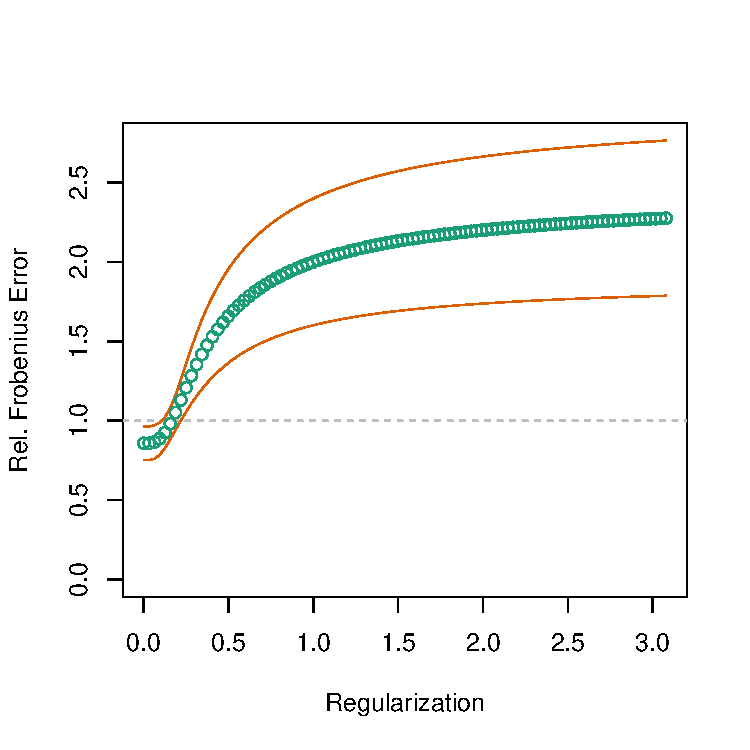
\includegraphics[scale=0.4]{plots/estimation-frob-s32-p020}}
  }
  \subfigure[$m/\mu = 2.0$]{
    \makebox{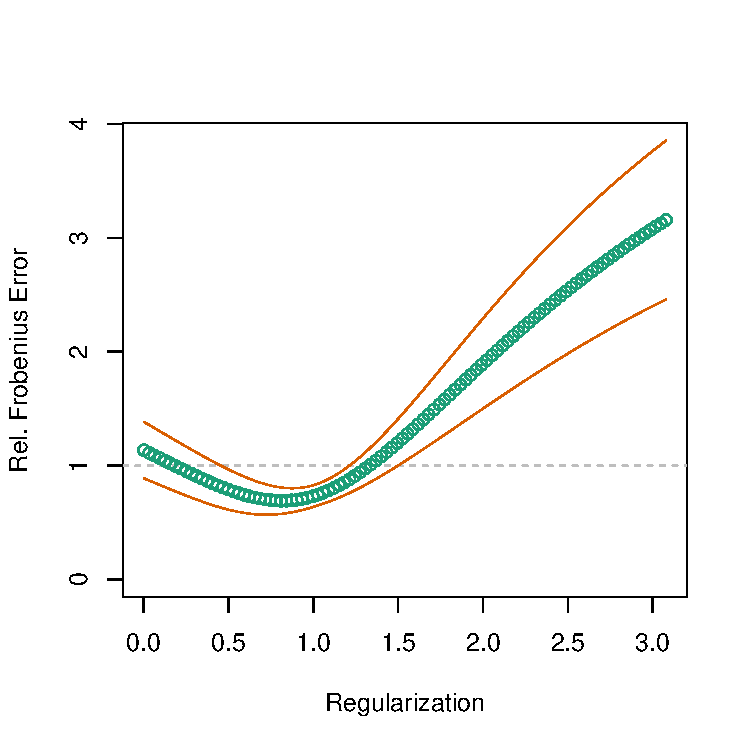
\includegraphics[scale=0.4]{plots/estimation-frob-s32-p200}}
  }
  \vspace{-1em}
  \caption{$s = 0$ edge swaps}
\end{figure}

\vspace{-2em}

\begin{figure}[h]
  \centering
  \subfigure[$m/\mu$ = 0.2]{
    \makebox{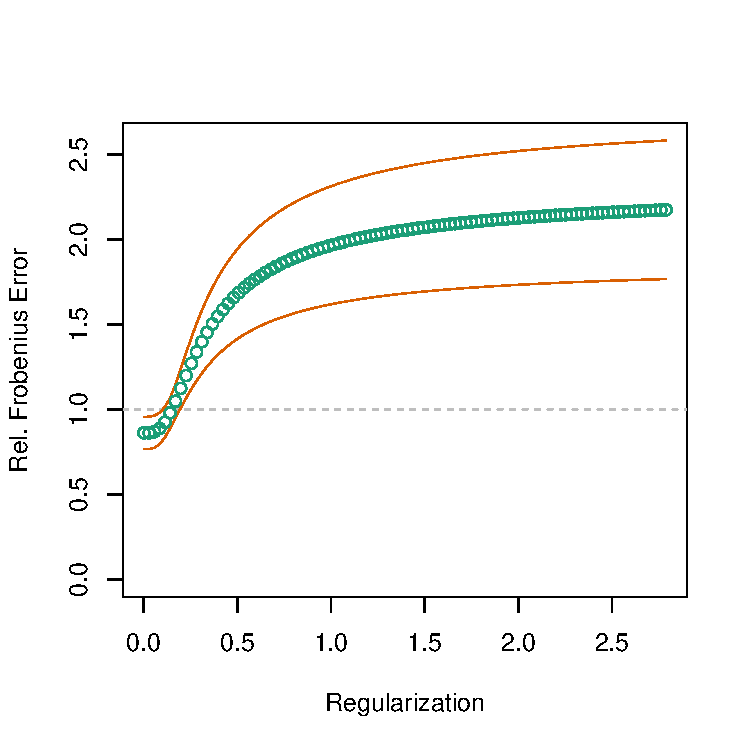
\includegraphics[scale=0.4]{plots/estimation-frob-p020}}
  }
  \subfigure[$m/\mu = 2.0$]{
    \makebox{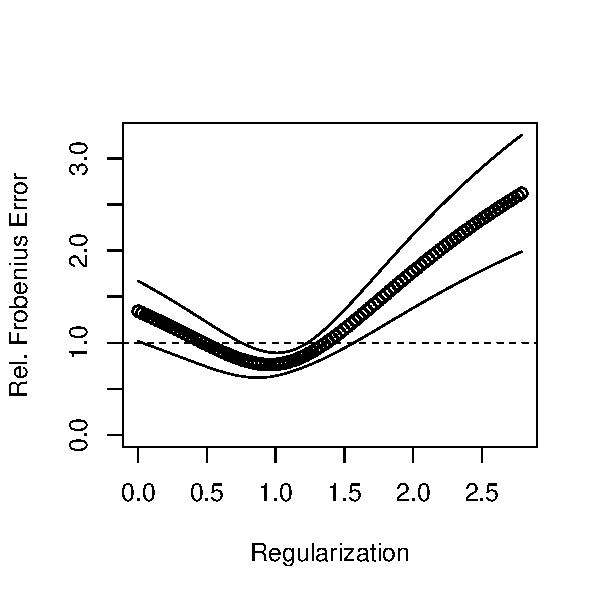
\includegraphics[scale=0.4]{plots/estimation-frob-p200}}
  }
  \vspace{-1em}
  \caption{$s = 4$ edge swaps}
\end{figure}

\vspace{-2em}

\begin{figure}[h]
  \centering
  \subfigure[$m/\mu$ = 0.2]{
    \makebox{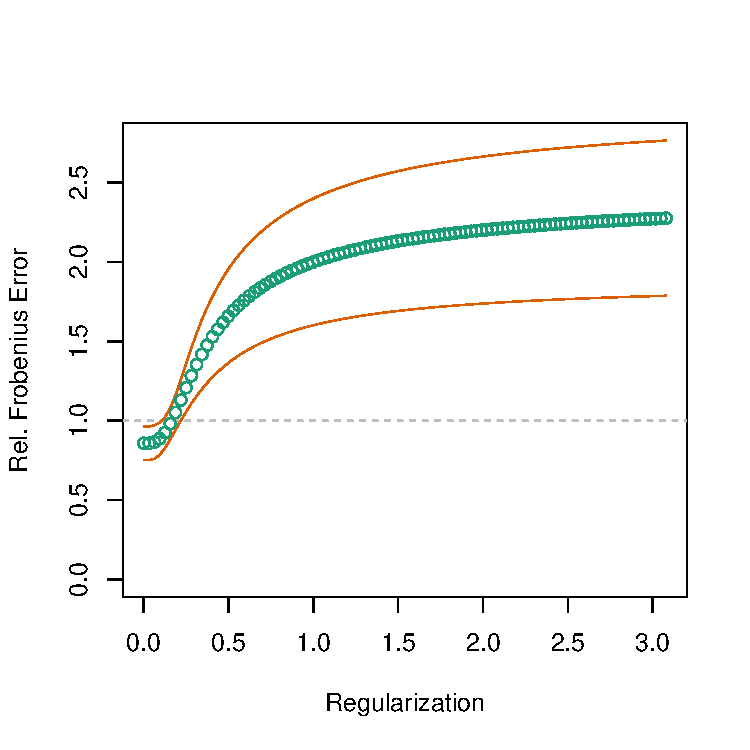
\includegraphics[scale=0.4]{plots/estimation-frob-s32-p020}}
  }
  \subfigure[$m/\mu = 2.0$]{
    \makebox{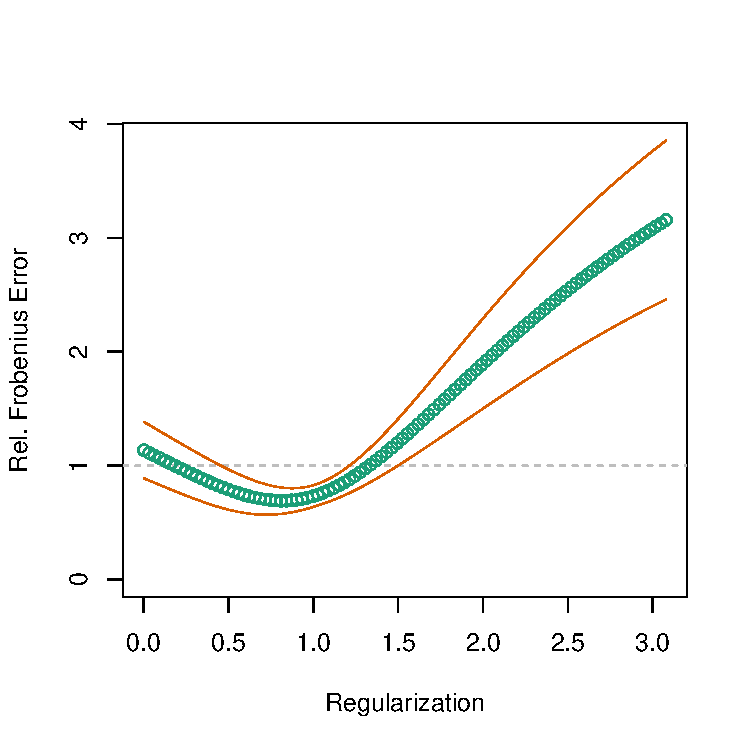
\includegraphics[scale=0.4]{plots/estimation-frob-s32-p200}}
  }
  \vspace{-1em}
  \caption{$s = 32$ edge swaps}
\end{figure}

\clearpage
\section{Supplementary Materials: Relative spectral error performance}
\label{S:spectral-peformance}

%\vspace{-2em}

\begin{figure}[h]
  \centering
  \subfigure[$m/\mu$ = 0.2]{
    \makebox{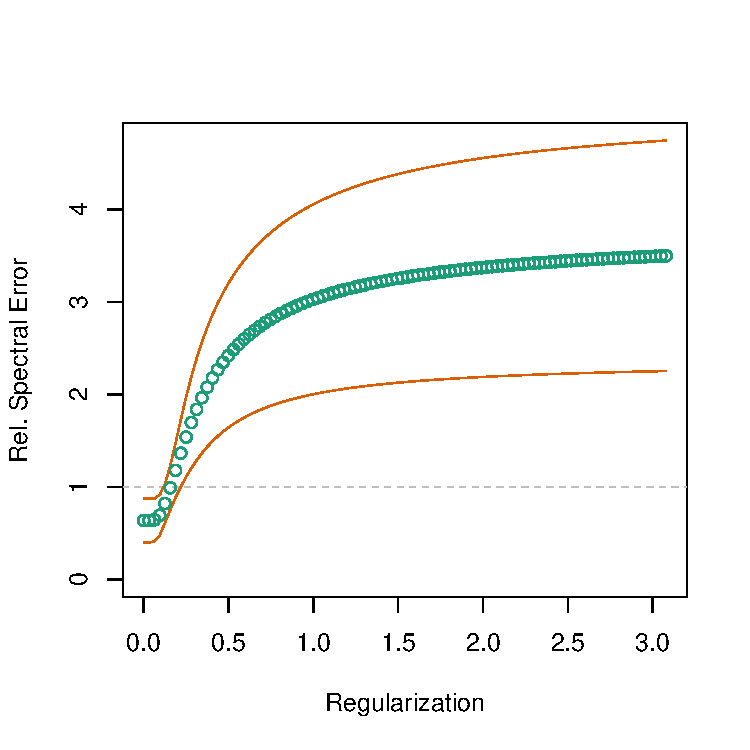
\includegraphics[scale=0.4]{plots/estimation-spec-s32-p020}}
  }
  \subfigure[$m/\mu = 2.0$]{
    \makebox{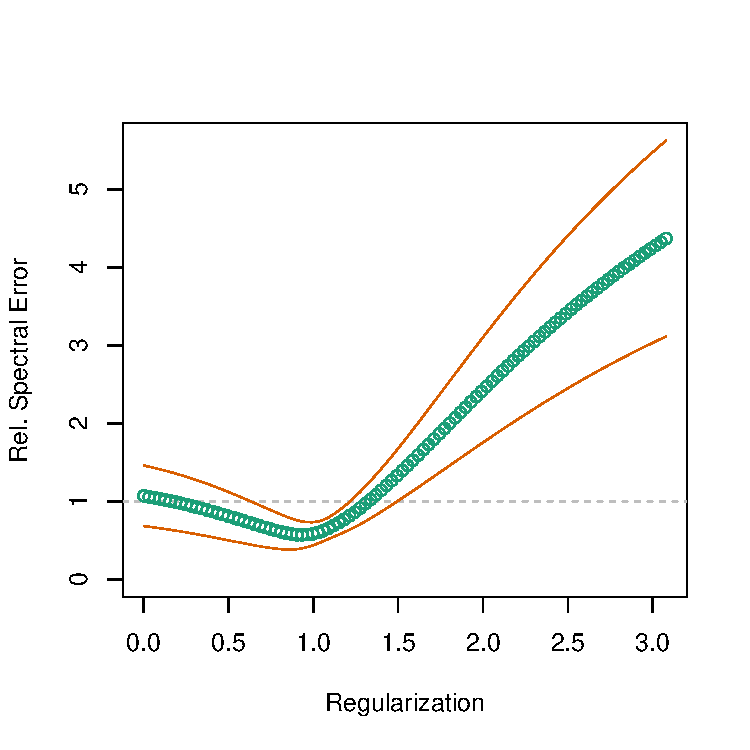
\includegraphics[scale=0.4]{plots/estimation-spec-s32-p200}}
  }
  \vspace{-1em}
  \caption{$s = 0$ edge swaps}
\end{figure}

\vspace{-2em}

\begin{figure}[h]
  \centering
  \subfigure[$m/\mu$ = 0.2]{
    \makebox{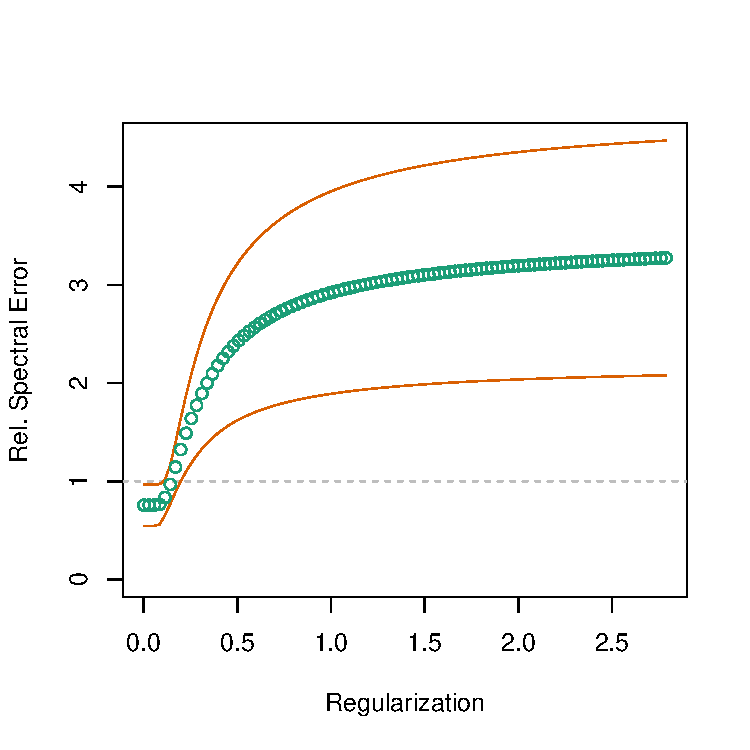
\includegraphics[scale=0.4]{plots/estimation-spec-p020}}
  }
  \subfigure[$m/\mu = 2.0$]{
    \makebox{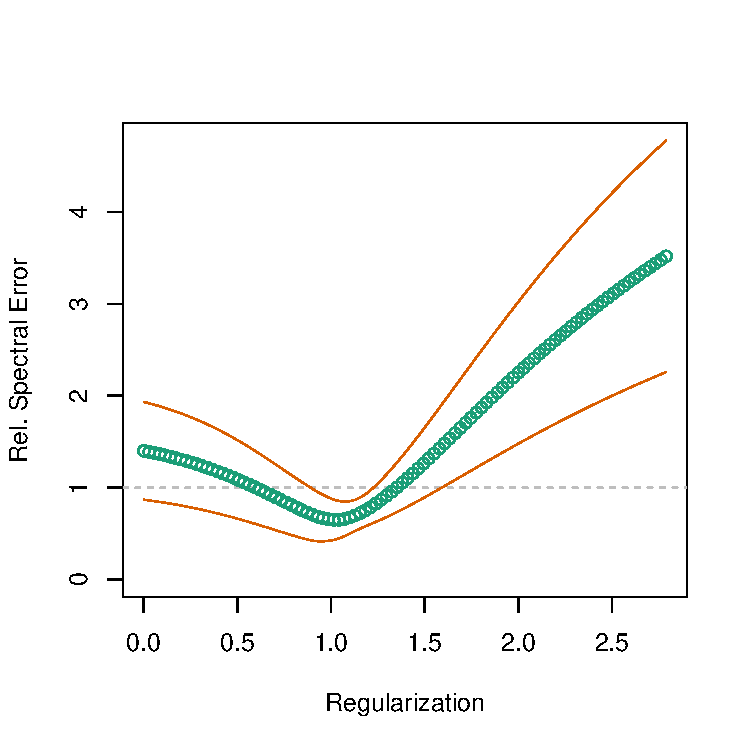
\includegraphics[scale=0.4]{plots/estimation-spec-p200}}
  }
  \vspace{-1em}
  \caption{$s = 4$ edge swaps}
\end{figure}

\vspace{-2em}

\begin{figure}[h]
  \centering
  \subfigure[$m/\mu$ = 0.2]{
    \makebox{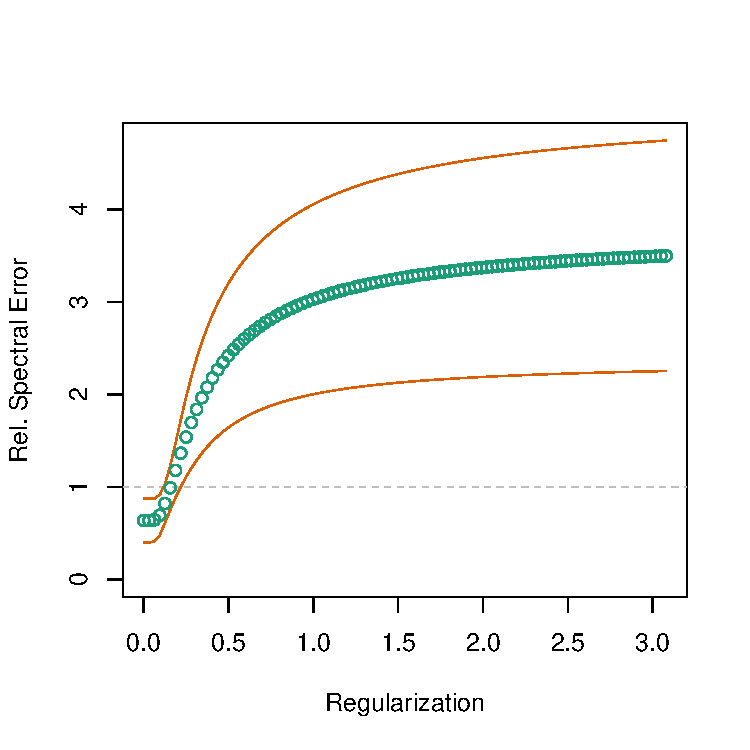
\includegraphics[scale=0.4]{plots/estimation-spec-s32-p020}}
  }
  \subfigure[$m/\mu = 2.0$]{
    \makebox{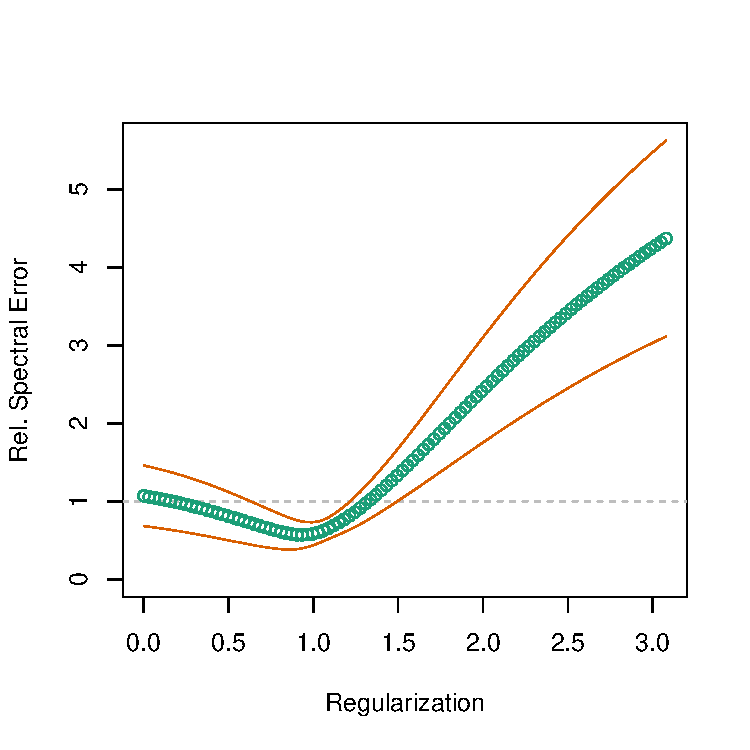
\includegraphics[scale=0.4]{plots/estimation-spec-s32-p200}}
  }
  \vspace{-1em}
  \caption{$s = 32$ edge swaps}
\end{figure}

\end{document}